\textit{Results from the JNI tests, FFT libraries and NEON optimizations are presented here.}

%%==================================================================
%% JNI-Tests
%%==================================================================
\section{JNI}
The results of the tests that measure the JNI overhead can be found in Table~\ref{tab:jni:common}. These tests are presented with block sizes defined in chapter \ref{ch:method} - Method. Execution time and confidence intervals are given in microseconds and are rounded to four decimal points. The number before the $\pm$ sign is the sample mean and the number after $\pm$ is a two sided confidence interval with a confidence level of $95\%$. Each test was executed 100 times to ensure that we get reliable sample means.

The test labeled \textbf{No params} is the test where a native void function with no parameters that returns immediately was called. \textbf{Vector} takes a \texttt{jdoubleArray} and returns a \texttt{jdoubleArray} immediately. \textbf{Convert} takes a \texttt{jdoubleArray}, converts it to a native array using \texttt{GetPrimitiveArrayCritical()}, converts it back to a \texttt{jdoubleArray} using \texttt{ReleasePrimitiveArrayCritical()} and returns a \texttt{jdoubleArray}. \textbf{Columbia} takes three \texttt{jdoubleArray}s, converts them the same way and returns the same way.

No surprising data regarding the first two tests were found. Neither the \textbf{No params} nor \textbf{Vector} tests had a clear increase in execution time for an increase in block size. \textbf{Vector} did have a higher mean for block size of \textbf{65536}. On the other hand, we can see that the 95\% confidence interval is very large ($\pm 3.1960$ \textmu s). This is due to its high standard deviation of 16.3058 \hilight{CITE}. Likewise, there is a spike in execution time mean for a block size of \textbf{1024} in the \textbf{Convert} test.


% DISCUSS HERE WHEN CORRECT DATA IS GATHERED
% As seen in Table \ref{tab:jni:common}, the execution times for calling the JNI varied in the range of one microseconds and 14 microseconds. \textbf{Columbia} with block size \textbf{6}

\begin{table}[H]
    \centering
    \caption{Results from the JNI tests, Time (\textmu s)}
    \label{tab:jni:common}
    \rowcolors{1}{}{lightgray}
\begin{tabular}{lrrrr}\toprule
\textbf{Block size}  & \textbf{No params} & \textbf{Vector} & \textbf{Convert} & \textbf{Columbia}\\\midrule
\textbf{16}  & 1.7922 $\pm$ 0.1392 & 1.9333 $\pm$ 0.1223 & 2.6052 $\pm$ 0.1004 & 4.1058 $\pm$ 0.3042\\
\textbf{32}  & 1.6983 $\pm$ 0.0220 & 2.8130 $\pm$ 1.7924 & 2.6006 $\pm$ 0.0370 & 3.9109 $\pm$ 0.0535\\
\textbf{64}  & 1.6755 $\pm$ 0.0149 & 1.6344 $\pm$ 0.1809 & 2.6630 $\pm$ 0.0425 & 3.9296 $\pm$ 0.0566\\
\textbf{128}  & 1.9604 $\pm$ 0.4978 & 1.2349 $\pm$ 0.1262 & 1.9375 $\pm$ 0.0843 & 3.0823 $\pm$ 0.0892\\
\textbf{256}  & 1.7292 $\pm$ 0.0694 & 1.3276 $\pm$ 0.2589 & 1.8141 $\pm$ 0.0276 & 3.0958 $\pm$ 0.0441\\
\textbf{512}  & 1.6916 $\pm$ 0.0110 & 1.2567 $\pm$ 0.1227 & 2.2818 $\pm$ 0.7011 & 3.1656 $\pm$ 0.0457\\
\textbf{1024}  & 2.0228 $\pm$ 0.5684 & 1.3167 $\pm$ 0.1341 & 6.3756 $\pm$ 8.4676 & 3.2896 $\pm$ 0.1396\\
\textbf{2048}  & 1.7218 $\pm$ 0.0288 & 1.5416 $\pm$ 0.1405 & 1.9099 $\pm$ 0.0898 & 3.4844 $\pm$ 0.1113\\
\textbf{4096}  & 1.1411 $\pm$ 0.0404 & 1.4010 $\pm$ 0.0788 & 2.0062 $\pm$ 0.1562 & 3.8562 $\pm$ 0.3197\\
\textbf{8192}  & 1.1105 $\pm$ 0.0078 & 1.4818 $\pm$ 0.0759 & 2.3671 $\pm$ 0.1897 & 3.8474 $\pm$ 0.4784\\
\textbf{16384}  & 1.1183 $\pm$ 0.0280 & 1.7308 $\pm$ 0.1043 & 2.5833 $\pm$ 0.1737 & 4.9724 $\pm$ 0.8955\\
\textbf{32768}  & 1.1162 $\pm$ 0.0084 & 2.2099 $\pm$ 0.1880 & 3.2062 $\pm$ 0.2029 & 5.3719 $\pm$ 0.2875\\
\textbf{65536}  & 1.7463 $\pm$ 1.2217 & 4.7474 $\pm$ 3.1960 & 4.3198 $\pm$ 0.2926 & 6.8136 $\pm$ 0.2499\\
\textbf{131072}  & 1.1027 $\pm$ 0.0141 & 2.6375 $\pm$ 0.1531 & 5.7004 $\pm$ 0.2681 & 9.6912 $\pm$ 1.4337\\
\textbf{262144} & 1.1006 $\pm$ 0.0118 & 3.3172 $\pm$ 0.1164 & 7.4630 $\pm$ 0.2309 & 10.2781 $\pm$ 0.2278\\
\bottomrule
\end{tabular}

\end{table}



%%==================================================================
%% FFT-Tests
%%==================================================================
\section{FFT Libraries}

The results from the FFT Libraries are presented in line graphs, both language specific and graphs with both Java and C++ are given to illustrate the differences between languages and also provide differences for specific languages clearly. The time unit for these tests are presented in milliseconds as opposed to microseconds that the JNI was measured in. This was because the FFT ran in ranges below one millisecond and above one second among different algorithms and different block sizes. The means are calculated from the results of 100 test runs.

\subsection{Float vs Double}

\subsection{Small block sizes}
Results from the small blocks tests shows clear difference between the different algorithms. In Figure~\ref{fig:all:line:small}, Princeton Recursive in Java perform the worst. Princeton Recursive in C++ and Princeton Iterative in Java perform better than Princeton Recursive Java although worse than the rest of the algorithms. % CHECK IF STILL RELEVANT AFTER NEW TESTS

% In Table ... we can see that the difference is statistically significant.

% found in Table~\ref{tab:cpp:small} and Table~\ref{tab:java:small}, shows that 


\begin{figure}
    \centering
    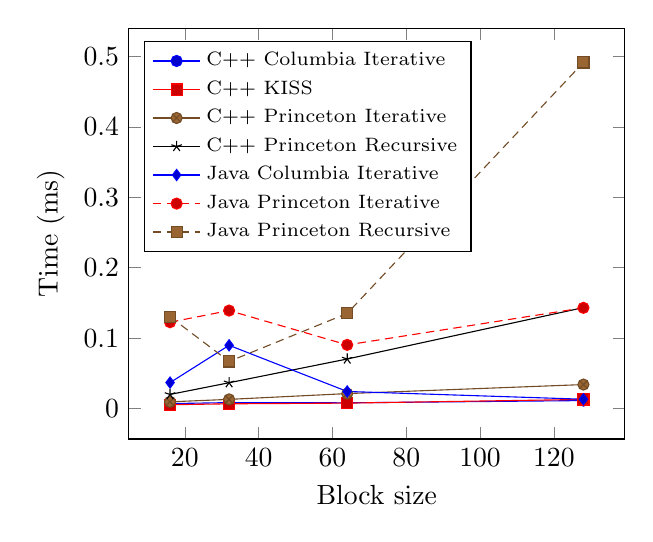
\begin{tikzpicture}
\begin{axis}[xlabel={Block size},ylabel={Time (ms)},width=0.65\linewidth,legend pos=north west,scaled y ticks = false,legend cell align=left,legend style={font=\scriptsize}]
\addplot coordinates {
(16, 0.0072)
(32, 0.0086)
(64, 0.0083)
(128, 0.0115)
};
\addplot coordinates {
(16, 0.0056)
(32, 0.0069)
(64, 0.0079)
(128, 0.0131)
};
\addplot coordinates {
(16, 0.0097)
(32, 0.0132)
(64, 0.0214)
(128, 0.0342)
};
\addplot coordinates {
(16, 0.0202)
(32, 0.0368)
(64, 0.0705)
(128, 0.1434)
};
\addplot coordinates {
(16, 0.0370)
(32, 0.0899)
(64, 0.0244)
(128, 0.0134)
};
\addplot coordinates {
(16, 0.1227)
(32, 0.1392)
(64, 0.0905)
(128, 0.1431)
};
\addplot coordinates {
(16, 0.1304)
(32, 0.0670)
(64, 0.1352)
(128, 0.4913)
};
\legend{C++ Columbia Iterative,C++ KISS,C++ Princeton Iterative,C++ Princeton Recursive,Java Columbia Iterative,Java Princeton Iterative,Java Princeton Recursive}
\end{axis}
\end{tikzpicture}

    \caption{Line graph for all algorithms, small block sizes}
    \label{fig:all:line:small}
\end{figure}

\begin{figure}
    \centering
    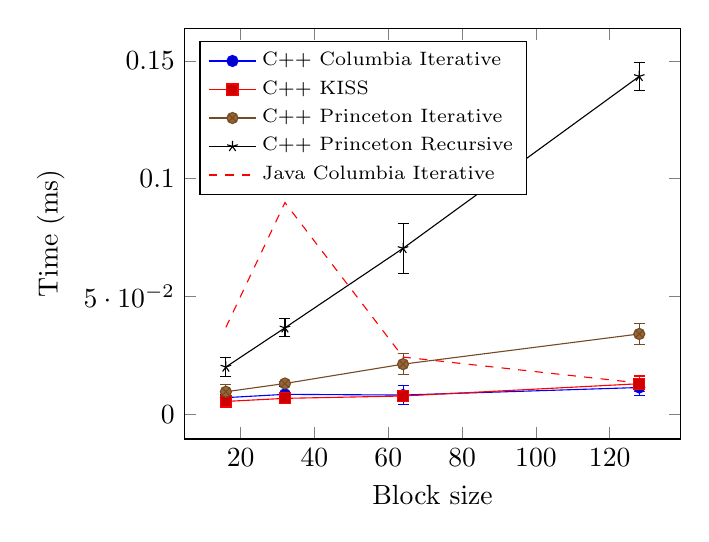
\begin{tikzpicture}
\begin{axis}[xlabel={Block size},ylabel={Time (ms)},width=0.65\linewidth,legend pos=north west,scaled y ticks = false,legend cell align=left,legend style={font=\scriptsize}]
\addplot+[error bars/.cd, y dir=both,y explicit] coordinates {
(16, 0.0072) +- (0.0012, 0.0012)
(32, 0.0086) +- (0.0034, 0.0034)
(64, 0.0083) +- (0.0041, 0.0041)
(128, 0.0115) +- (0.0033, 0.0033)
};
\addplot+[error bars/.cd, y dir=both,y explicit] coordinates {
(16, 0.0056) +- (0.0013, 0.0013)
(32, 0.0069) +- (0.0005, 0.0005)
(64, 0.0079) +- (0.0009, 0.0009)
(128, 0.0131) +- (0.0033, 0.0033)
};
\addplot+[error bars/.cd, y dir=both,y explicit] coordinates {
(16, 0.0097) +- (0.0032, 0.0032)
(32, 0.0132) +- (0.0009, 0.0009)
(64, 0.0214) +- (0.0044, 0.0044)
(128, 0.0342) +- (0.0045, 0.0045)
};
\addplot+[error bars/.cd, y dir=both,y explicit] coordinates {
(16, 0.0202) +- (0.0039, 0.0039)
(32, 0.0368) +- (0.0038, 0.0038)
(64, 0.0705) +- (0.0105, 0.0105)
(128, 0.1434) +- (0.0059, 0.0059)
};
\addplot+[style=dashed,color=red,mark=none] coordinates {
(16, 0.0370) +- (0.0055, 0.0055)
(32, 0.0899) +- (0.0169, 0.0169)
(64, 0.0244) +- (0.0637, 0.0637)
(128, 0.0134) +- (0.0005, 0.0005)
};
\legend{C++ Columbia Iterative , C++ KISS , C++ Princeton Iterative , C++ Princeton Recursive, Java Columbia Iterative}
\end{axis}
\end{tikzpicture}

    \caption{C++ line graph for small block sizes}
    \label{fig:cpp:line:small}
\end{figure}
\begin{table}
    \centering
    \caption{C++ results table for small block sizes}
    \label{tab:cpp:small}
    \resizebox{\columnwidth}{!}{
        \rowcolors{1}{}{lightgray}
\begin{tabular}{lrrrr}\toprule
\textbf{Block size}  & \textbf{Columbia Iterative} & \textbf{KISS} & \textbf{Princeton Iterative} & \textbf{Princeton Recursive}\\\midrule
\textbf{16}  & 0.007 $\pm$ 0.0002 & 0.005 $\pm$ 0.0002 & 0.009 $\pm$ 0.0006 & 0.020 $\pm$ 0.0008\\
\textbf{32}  & 0.008 $\pm$ 0.0006 & 0.006 $\pm$ 0.0002 & 0.013 $\pm$ 0.0002 & 0.036 $\pm$ 0.0008\\
\textbf{64}  & 0.008 $\pm$ 0.0008 & 0.007 $\pm$ 0.0002 & 0.021 $\pm$ 0.0008 & 0.070 $\pm$ 0.0022\\
\textbf{128} & 0.011 $\pm$ 0.0006 & 0.013 $\pm$ 0.0006 & 0.034 $\pm$ 0.0008 & 0.143 $\pm$ 0.0012\\
\bottomrule
\end{tabular}

    }
\end{table}


\begin{figure}
    \centering
    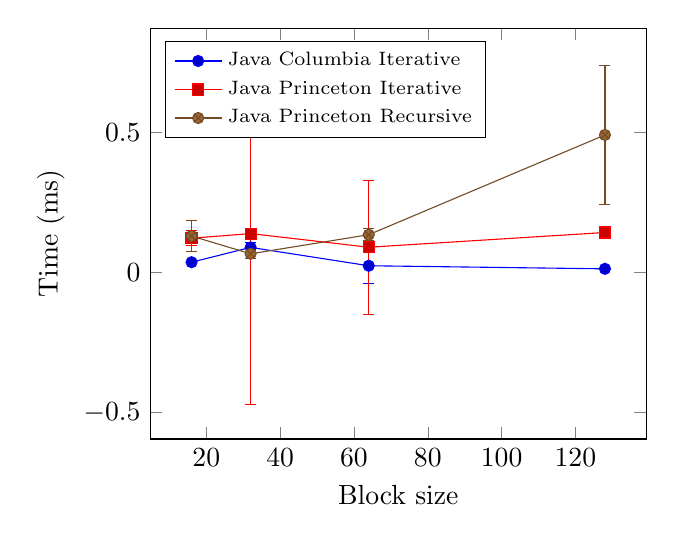
\begin{tikzpicture}
\begin{axis}[xlabel={Block size},ylabel={Time (ms)},width=0.65\linewidth,legend pos=north west,scaled y ticks = false,legend cell align=left,legend style={font=\scriptsize}]
\addplot+[error bars/.cd, y dir=both,y explicit] coordinates {
(16, 0.0370) +- (0.0055, 0.0055)
(32, 0.0899) +- (0.0169, 0.0169)
(64, 0.0244) +- (0.0637, 0.0637)
(128, 0.0134) +- (0.0005, 0.0005)
};
\addplot+[error bars/.cd, y dir=both,y explicit] coordinates {
(16, 0.1227) +- (0.0268, 0.0268)
(32, 0.1392) +- (0.6110, 0.6110)
(64, 0.0905) +- (0.2393, 0.2393)
(128, 0.1431) +- (0.0097, 0.0097)
};
\addplot+[error bars/.cd, y dir=both,y explicit] coordinates {
(16, 0.1304) +- (0.0546, 0.0546)
(32, 0.0670) +- (0.0177, 0.0177)
(64, 0.1352) +- (0.0215, 0.0215)
(128, 0.4913) +- (0.2475, 0.2475)
};
\legend{Java Columbia Iterative , Java Princeton Iterative , Java Princeton Recursive}
\end{axis}
\end{tikzpicture}

    \caption{Java line graph for small block sizes}
    \label{fig:java:line:small}
\end{figure}
\begin{table}
    \centering
    \caption{Java results table for small block sizes}
    \label{tab:java:small}
    \resizebox{\columnwidth}{!}{
        \rowcolors{1}{}{lightgray}
\begin{tabular}{lccc}\toprule
\textbf{Block size}  & \textbf{Columbia Iterative} & \textbf{Princeton Iterative} & \textbf{Princeton Recursive}\\\midrule
\textbf{16}  & 0.0370 $\pm$ 0.0010 & 0.1227 $\pm$ 0.0053 & 0.1304 $\pm$ 0.0108\\
\textbf{32}  & 0.0899 $\pm$ 0.0033 & 0.1392 $\pm$ 0.1198 & 0.0670 $\pm$ 0.0035\\
\textbf{64}  & 0.0244 $\pm$ 0.0125 & 0.0905 $\pm$ 0.0468 & 0.1352 $\pm$ 0.0043\\
\textbf{128} & 0.0134 $\pm$ 0.0002 & 0.1431 $\pm$ 0.0020 & 0.4913 $\pm$ 0.0486\\
\bottomrule
\end{tabular}

    }
\end{table}

\subsection{Medium block sizes}
\begin{figure}
    \centering
    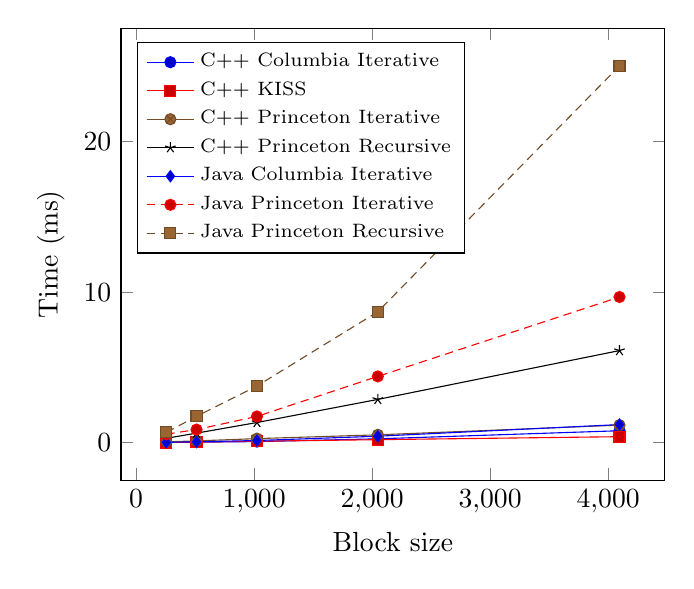
\begin{tikzpicture}
\begin{axis}[xlabel={Block size},ylabel={Time (ms)},width=0.70\linewidth,legend pos=north west,scaled y ticks = false,legend cell align=left,legend style={font=\scriptsize}]
\addplot coordinates {
(256, 0.0200)
(512, 0.0366)
(1024, 0.0773)
(2048, 0.2604)
(4096, 0.7974)
};
\addplot coordinates {
(256, 0.0182)
(512, 0.0461)
(1024, 0.0992)
(2048, 0.2047)
(4096, 0.4022)
};
\addplot coordinates {
(256, 0.0627)
(512, 0.1225)
(1024, 0.2744)
(2048, 0.5257)
(4096, 1.1701)
};
\addplot coordinates {
(256, 0.2978)
(512, 0.6379)
(1024, 1.3437)
(2048, 2.8773)
(4096, 6.1206)
};
\addplot coordinates {
(256, 0.0293)
(512, 0.0615)
(1024, 0.1484)
(2048, 0.4338)
(4096, 1.2071)
};
\addplot coordinates {
(256, 0.5698)
(512, 0.8758)
(1024, 1.7488)
(2048, 4.4055)
(4096, 9.6792)
};
\addplot coordinates {
(256, 0.6929)
(512, 1.7515)
(1024, 3.7688)
(2048, 8.6983)
(4096, 25.0276)
};
\legend{C++ Columbia Iterative,C++ KISS,C++ Princeton Iterative,C++ Princeton Recursive,Java Columbia Iterative,Java Princeton Iterative,Java Princeton Recursive}
\end{axis}
\end{tikzpicture}

    \caption{Line graph for all algorithms, medium block sizes}
    \label{fig:all:line:medium}
\end{figure}

\begin{figure}
    \centering
    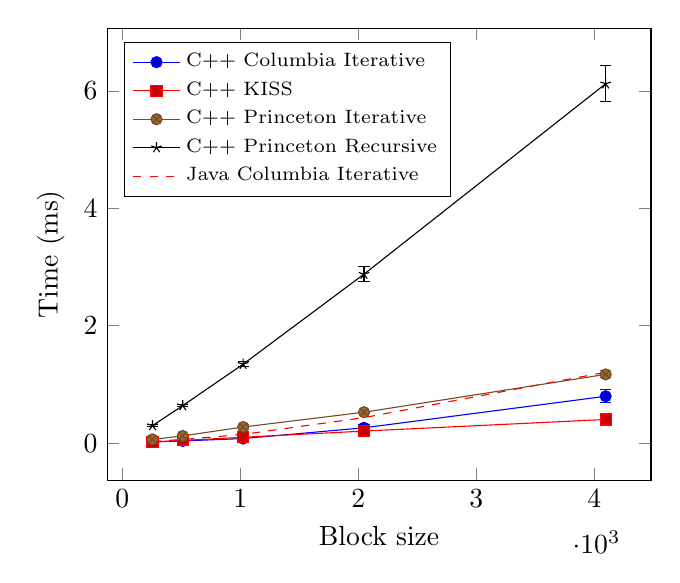
\begin{tikzpicture}
\begin{axis}[xlabel={Block size},ylabel={Time (ms)},width=0.70\linewidth,legend pos=north west,scaled x ticks={base 10:-3},legend cell align=left,legend style={font=\scriptsize}]
\addplot+[error bars/.cd, y dir=both,y explicit] coordinates {
(256, 0.0200) +- (0.0043, 0.0043)
(512, 0.0366) +- (0.0033, 0.0033)
(1024, 0.0773) +- (0.0097, 0.0097)
(2048, 0.2604) +- (0.0634, 0.0634)
(4096, 0.7974) +- (0.1097, 0.1097)
};
\addplot+[error bars/.cd, y dir=both,y explicit] coordinates {
(256, 0.0182) +- (0.0037, 0.0037)
(512, 0.0461) +- (0.0110, 0.0110)
(1024, 0.0992) +- (0.0883, 0.0883)
(2048, 0.2047) +- (0.0765, 0.0765)
(4096, 0.4022) +- (0.0625, 0.0625)
};
\addplot+[error bars/.cd, y dir=both,y explicit] coordinates {
(256, 0.0627) +- (0.0040, 0.0040)
(512, 0.1225) +- (0.0032, 0.0032)
(1024, 0.2744) +- (0.0495, 0.0495)
(2048, 0.5257) +- (0.0185, 0.0185)
(4096, 1.1701) +- (0.0602, 0.0602)
};
\addplot+[error bars/.cd, y dir=both,y explicit] coordinates {
(256, 0.2978) +- (0.0127, 0.0127)
(512, 0.6379) +- (0.0181, 0.0181)
(1024, 1.3437) +- (0.0445, 0.0445)
(2048, 2.8773) +- (0.1288, 0.1288)
(4096, 6.1206) +- (0.3046, 0.3046)
};
\addplot+[style=dashed,color=red,mark=none] coordinates {
(256, 0.0293) +- (0.0042, 0.0042)
(512, 0.0615) +- (0.0047, 0.0047)
(1024, 0.1484) +- (0.0308, 0.0308)
(2048, 0.4338) +- (0.0806, 0.0806)
(4096, 1.2071) +- (0.1807, 0.1807)
};
\legend{C++ Columbia Iterative , C++ KISS , C++ Princeton Iterative , C++ Princeton Recursive, Java Columbia Iterative}
\end{axis}
\end{tikzpicture}

    \caption{C++ line graph for medium block sizes}
    \label{fig:cpp:line:medium}
\end{figure}
\begin{table}
    \centering
    \caption{C++ results table for small block sizes}
    \label{tab:cpp:medium}
    \resizebox{\columnwidth}{!}{
        \rowcolors{1}{}{lightgray}
\begin{tabular}{lrrrr}\toprule
\textbf{Block size}  & \textbf{Columbia Iterative} & \textbf{KISS} & \textbf{Princeton Iterative} & \textbf{Princeton Recursive}\\\midrule
\textbf{256}  & 0.02 $\pm$ 0.0008 & 0.01 $\pm$ 0.0008 & 0.06 $\pm$ 0.0008 & 0.29 $\pm$ 0.0025\\
\textbf{512}  & 0.03 $\pm$ 0.0006 & 0.04 $\pm$ 0.0022 & 0.12 $\pm$ 0.0006 & 0.63 $\pm$ 0.0035\\
\textbf{1024}  & 0.07 $\pm$ 0.0020 & 0.09 $\pm$ 0.0172 & 0.27 $\pm$ 0.0098 & 1.34 $\pm$ 0.0086\\
\textbf{2048}  & 0.26 $\pm$ 0.0123 & 0.20 $\pm$ 0.0149 & 0.52 $\pm$ 0.0035 & 2.87 $\pm$ 0.0253\\
\textbf{4096} & 0.79 $\pm$ 0.0216 & 0.40 $\pm$ 0.0123 & 1.17 $\pm$ 0.0118 & 6.12 $\pm$ 0.0598\\
\bottomrule
\end{tabular}

    }
\end{table}


\begin{figure}
    \centering
    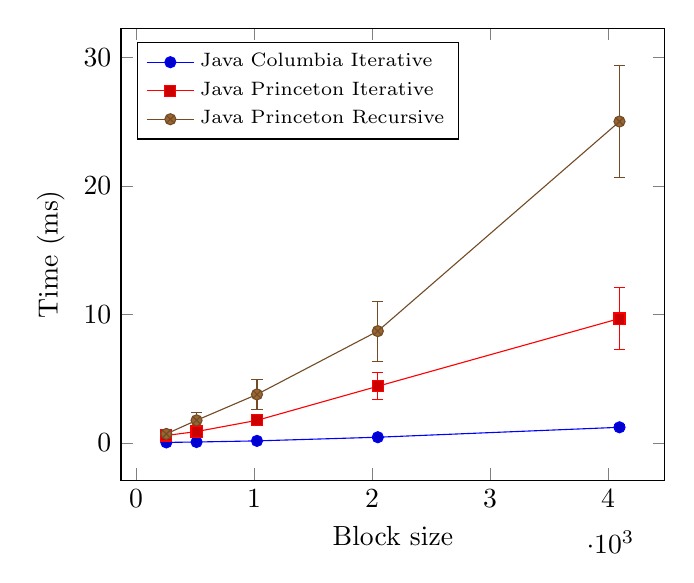
\begin{tikzpicture}
\begin{axis}[xlabel={Block size},ylabel={Time (ms)},width=0.70\linewidth,legend pos=north west,scaled x ticks={base 10:-3},legend cell align=left,legend style={font=\scriptsize}]
\addplot+[error bars/.cd, y dir=both,y explicit] coordinates {
(256, 0.0293) +- (0.0042, 0.0042)
(512, 0.0615) +- (0.0047, 0.0047)
(1024, 0.1484) +- (0.0308, 0.0308)
(2048, 0.4338) +- (0.0806, 0.0806)
(4096, 1.2071) +- (0.1807, 0.1807)
};
\addplot+[error bars/.cd, y dir=both,y explicit] coordinates {
(256, 0.5698) +- (0.4834, 0.4834)
(512, 0.8758) +- (0.3145, 0.3145)
(1024, 1.7488) +- (0.3452, 0.3452)
(2048, 4.4055) +- (1.0527, 1.0527)
(4096, 9.6792) +- (2.3947, 2.3947)
};
\addplot+[error bars/.cd, y dir=both,y explicit] coordinates {
(256, 0.6929) +- (0.1662, 0.1662)
(512, 1.7515) +- (0.6352, 0.6352)
(1024, 3.7688) +- (1.1879, 1.1879)
(2048, 8.6983) +- (2.3341, 2.3341)
(4096, 25.0276) +- (4.3322, 4.3322)
};
\legend{Java Columbia Iterative , Java Princeton Iterative , Java Princeton Recursive}
\end{axis}
\end{tikzpicture}

    \caption{Java line graph for medium block sizes}
    \label{fig:java:line:medium}
\end{figure}
\begin{table}
    \centering
    \caption{Java results table for medium block sizes}
    \label{tab:java:medium}
    \rowcolors{1}{}{lightgray}
\begin{tabular}{lccc}\toprule
\textbf{Block size}  & \textbf{Columbia Iterative} & \textbf{Princeton Iterative} & \textbf{Princeton Recursive}\\\midrule
\textbf{256}  & 0.0293 $\pm$ 0.0008 & 0.5698 $\pm$ 0.0947 & 0.6929 $\pm$ 0.0325\\
\textbf{512}  & 0.0615 $\pm$ 0.0010 & 0.8758 $\pm$ 0.0615 & 1.7515 $\pm$ 0.1245\\
\textbf{1024}  & 0.1484 $\pm$ 0.0061 & 1.7488 $\pm$ 0.0676 & 3.7688 $\pm$ 0.2328\\
\textbf{2048}  & 0.4338 $\pm$ 0.0159 & 4.4055 $\pm$ 0.2064 & 8.6983 $\pm$ 0.4575\\
\textbf{4096} & 1.2071 $\pm$ 0.0355 & 9.6792 $\pm$ 0.4694 & 25.0276 $\pm$ 0.8491\\
\bottomrule
\end{tabular}

\end{table}

\subsection{Large block sizes}

\begin{figure}
    \centering
    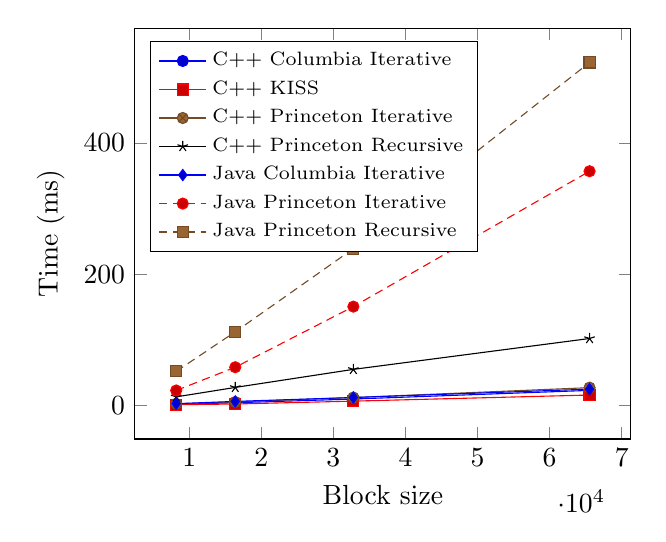
\begin{tikzpicture}
\begin{axis}[xlabel={Block size},ylabel={Time (ms)},width=0.65\linewidth,legend pos=north west,scaled y ticks = false,legend cell align=left,legend style={font=\scriptsize}]
\addplot coordinates {
(8192, 1.9326)
(16384, 4.2789)
(32768, 9.9388)
(65536, 23.1031)
};
\addplot coordinates {
(8192, 1.2470)
(16384, 2.3713)
(32768, 6.7420)
(65536, 16.0281)
};
\addplot coordinates {
(8192, 2.5845)
(16384, 5.4518)
(32768, 12.2266)
(65536, 27.2805)
};
\addplot coordinates {
(8192, 13.2345)
(16384, 27.6080)
(32768, 55.1227)
(65536, 102.1585)
};
\addplot coordinates {
(8192, 2.8726)
(16384, 6.3214)
(32768, 12.2634)
(65536, 24.9874)
};
\addplot coordinates {
(8192, 22.9609)
(16384, 58.3825)
(32768, 150.7299)
(65536, 356.9871)
};
\addplot coordinates {
(8192, 52.0853)
(16384, 112.3024)
(32768, 239.0777)
(65536, 522.7409)
};
\legend{C++ Columbia Iterative,C++ KISS,C++ Princeton Iterative,C++ Princeton Recursive,Java Columbia Iterative,Java Princeton Iterative,Java Princeton Recursive}
\end{axis}
\end{tikzpicture}

    \caption{Line graph for all algorithms, large block sizes}
    \label{fig:all:line:large}
\end{figure}

\begin{figure}
    \centering
    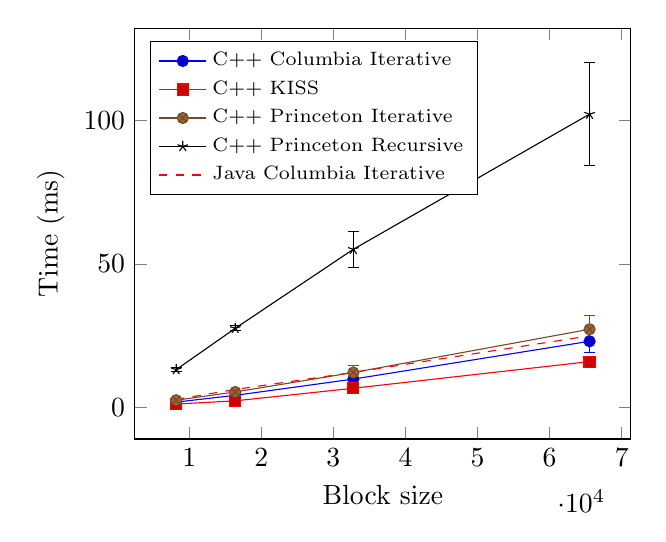
\begin{tikzpicture}
\begin{axis}[xlabel={Block size},ylabel={Time (ms)},width=0.65\linewidth,legend pos=north west,scaled y ticks = false,legend cell align=left,legend style={font=\scriptsize}]
\addplot+[error bars/.cd, y dir=both,y explicit] coordinates {
(8192, 1.9326) +- (0.2654, 0.2654)
(16384, 4.2789) +- (0.6399, 0.6399)
(32768, 9.9388) +- (1.6341, 1.6341)
(65536, 23.1031) +- (3.9019, 3.9019)
};
\addplot+[error bars/.cd, y dir=both,y explicit] coordinates {
(8192, 1.2470) +- (0.2301, 0.2301)
(16384, 2.3713) +- (0.4915, 0.4915)
(32768, 6.7420) +- (1.2931, 1.2931)
(65536, 16.0281) +- (1.8073, 1.8073)
};
\addplot+[error bars/.cd, y dir=both,y explicit] coordinates {
(8192, 2.5845) +- (0.2085, 0.2085)
(16384, 5.4518) +- (0.5858, 0.5858)
(32768, 12.2266) +- (2.4651, 2.4651)
(65536, 27.2805) +- (4.8616, 4.8616)
};
\addplot+[error bars/.cd, y dir=both,y explicit] coordinates {
(8192, 13.2345) +- (0.7311, 0.7311)
(16384, 27.6080) +- (0.9098, 0.9098)
(32768, 55.1227) +- (6.2636, 6.2636)
(65536, 102.1585) +- (17.9911, 17.9911)
};
\addplot+[style=dashed,color=red,mark=none] coordinates {
(8192, 2.8726) +- (0.3247, 0.3247)
(16384, 6.3214) +- (1.0542, 1.0542)
(32768, 12.2634) +- (2.9076, 2.9076)
(65536, 24.9874) +- (4.6266, 4.6266)
};
\legend{C++ Columbia Iterative , C++ KISS , C++ Princeton Iterative , C++ Princeton Recursive, Java Columbia Iterative}
\end{axis}
\end{tikzpicture}

    \caption{C++ line graph for large block sizes}
    \label{fig:cpp:line:large}
\end{figure}
\begin{table}
    \centering
    \caption{C++ results table for large block sizes}
    \label{tab:cpp:large}
    \resizebox{\columnwidth}{!}{
        \rowcolors{1}{}{lightgray}
\begin{tabular}{lrrrr}\toprule
\textbf{Block size}  & \textbf{Columbia Iterative} & \textbf{KISS} & \textbf{Princeton Iterative} & \textbf{Princeton Recursive}\\\midrule
\textbf{8192}  & 1.9326 $\pm$ 0.0519 & 1.2470 $\pm$ 0.0451 & 2.5845 $\pm$ 0.0410 & 13.2345 $\pm$ 0.1433\\
\textbf{16384}  & 4.2789 $\pm$ 0.1254 & 2.3713 $\pm$ 0.0962 & 5.4518 $\pm$ 0.1149 & 27.6080 $\pm$ 0.1784\\
\textbf{32768}  & 9.9388 $\pm$ 0.3203 & 6.7420 $\pm$ 0.2534 & 12.2266 $\pm$ 0.4831 & 55.1227 $\pm$ 1.2277\\
\textbf{65536} & 23.1031 $\pm$ 0.7648 & 16.0281 $\pm$ 0.3542 & 27.2805 $\pm$ 0.9530 & 102.1585 $\pm$ 3.5262\\
\bottomrule
\end{tabular}

    }
\end{table}


\begin{figure}
    \centering
    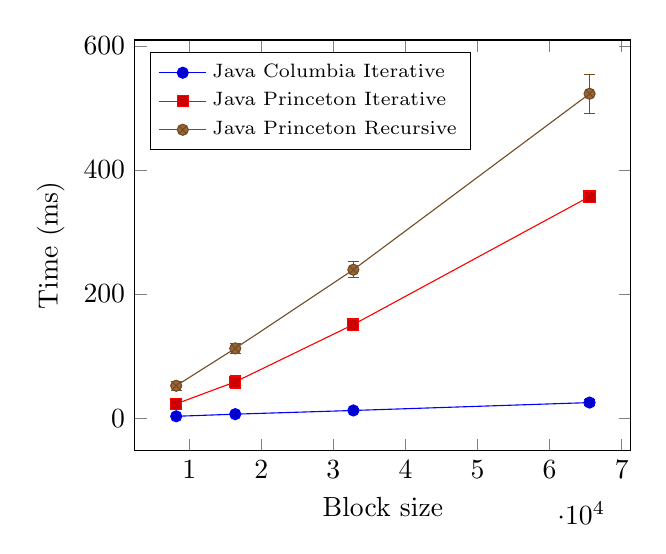
\begin{tikzpicture}
\begin{axis}[xlabel={Block size},ylabel={Time (ms)},width=0.65\linewidth,legend pos=north west,legend cell align=left,legend style={font=\scriptsize}]
\addplot+[error bars/.cd, y dir=both,y explicit] coordinates {
(8192, 2.8726) +- (0.3247, 0.3247)
(16384, 6.3214) +- (1.0542, 1.0542)
(32768, 12.2634) +- (2.9076, 2.9076)
(65536, 24.9874) +- (4.6266, 4.6266)
};
\addplot+[error bars/.cd, y dir=both,y explicit] coordinates {
(8192, 22.9609) +- (5.6248, 5.6248)
(16384, 58.3825) +- (9.9410, 9.9410)
(32768, 150.7299) +- (5.5432, 5.5432)
(65536, 356.9871) +- (8.0942, 8.0942)
};
\addplot+[error bars/.cd, y dir=both,y explicit] coordinates {
(8192, 52.0853) +- (7.1292, 7.1292)
(16384, 112.3024) +- (8.1890, 8.1890)
(32768, 239.0777) +- (12.8962, 12.8962)
(65536, 522.7409) +- (31.4586, 31.4586)
};
\legend{Java Columbia Iterative , Java Princeton Iterative , Java Princeton Recursive}
\end{axis}
\end{tikzpicture}

    \caption{Java line graph for large block sizes}
    \label{fig:java:line:large}
\end{figure}
\begin{table}
    \centering
    \caption{Java results table for large block sizes}
    \label{tab:java:large}
    \rowcolors{1}{}{lightgray}
\begin{tabular}{lccc}\toprule
\textbf{Block size}  & \textbf{Columbia Iterative} & \textbf{Princeton Iterative} & \textbf{Princeton Recursive}\\\midrule
\textbf{8192}  & 2.8726 $\pm$ 0.0637 & 22.9609 $\pm$ 1.1025 & 52.0853 $\pm$ 1.3973\\
\textbf{16384}  & 6.3214 $\pm$ 0.2066 & 58.3825 $\pm$ 1.9484 & 112.3024 $\pm$ 1.6050\\
\textbf{32768}  & 12.2634 $\pm$ 0.5700 & 150.7299 $\pm$ 1.0864 & 239.0777 $\pm$ 2.5276\\
\textbf{65536} & 24.9874 $\pm$ 0.9069 & 356.9871 $\pm$ 1.5864 & 522.7409 $\pm$ 6.1660\\
\bottomrule
\end{tabular}

\end{table}


% Which is slowest and why (discussion)??

% Which is fastest and why (discussion)??

% Which tests triggered the GC??

%%==================================================================
%% NEON-Tests
%%==================================================================
\section{Optimizations}

\begin{table}
    \centering
    \caption{Java results table for extra large block sizes}
    \label{tab:java:extra}
    \rowcolors{1}{}{lightgray}
\begin{tabular}{lrrr}\toprule
\textbf{Block size}  & \textbf{Columbia Iterative} & \textbf{Princeton Iterative} & \textbf{Princeton Recursive}\\\midrule
\textbf{8192}  & 2.87 $\pm$ 0.06 & 22.96 $\pm$ 1.10 & 52.08 $\pm$ 1.39\\
\textbf{16384}  & 6.32 $\pm$ 0.20 & 58.38 $\pm$ 1.94 & 112.30 $\pm$ 1.60\\
\textbf{32768}  & 12.26 $\pm$ 0.57 & 150.72 $\pm$ 1.08 & 239.07 $\pm$ 2.52\\
\textbf{65536}  & 24.98 $\pm$ 0.90 & 356.98 $\pm$ 1.58 & 522.74 $\pm$ 6.16\\
\textbf{131072}  & 85.94 $\pm$ 1.60 & 815.86 $\pm$ 3.43 & 1144.88 $\pm$ 17.87\\
\textbf{262144} & 274.51 $\pm$ 5.11 & 2108.07 $\pm$ 27.53 & 2638.05 $\pm$ 40.54\\
\bottomrule
\end{tabular}

\end{table}

\begin{figure}
    \centering
    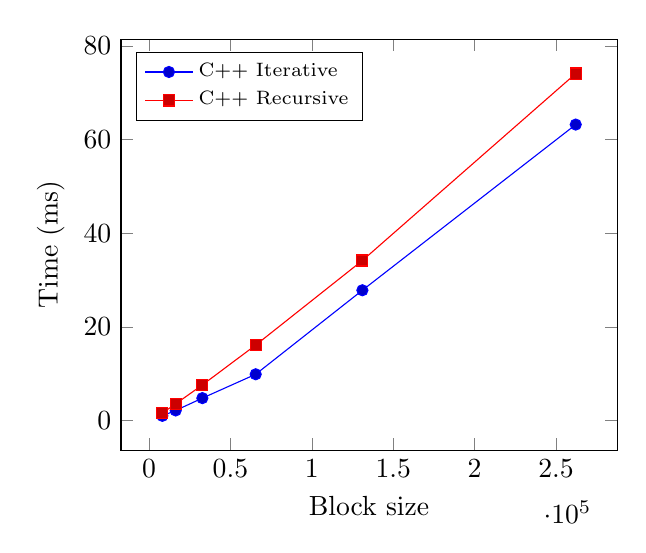
\begin{tikzpicture}
\begin{axis}[xlabel={Block size},ylabel={Time (ms)},width=0.65\linewidth,legend pos=north west,scaled y ticks = false,legend cell align=left,legend style={font=\scriptsize}]
\addplot coordinates {
(8192, 1.0051)
(16384, 2.1559)
(32768, 4.7898)
(65536, 9.8807)
(131072, 27.8158)
(262144, 63.1858)
};
\addplot coordinates {
(8192, 1.6133)
(16384, 3.5690)
(32768, 7.6009)
(65536, 16.1129)
(131072, 34.1650)
(262144, 74.0746)
};
\legend{C++ Iterative,C++ Recursive}
\end{axis}
\end{tikzpicture}

    \caption{NEON results table for extra large block sizes}
    \label{fig:neon:line:extra}
\end{figure}

\begin{table}
    \centering
    \rowcolors{1}{}{lightgray}
\begin{tabular}{lrr}\toprule
\textbf{Block size}  & \textbf{Iterative} & \textbf{Recursive}\\\midrule
\textbf{8192}  & 1.00 $\pm$ 0.01 & 1.61 $\pm$ 0.02\\
\textbf{16384}  & 2.15 $\pm$ 0.05 & 3.56 $\pm$ 0.08\\
\textbf{32768}  & 4.78 $\pm$ 0.15 & 7.60 $\pm$ 0.18\\
\textbf{65536}  & 9.88 $\pm$ 0.24 & 16.11 $\pm$ 0.37\\
\textbf{131072}  & 27.81 $\pm$ 0.71 & 34.16 $\pm$ 0.47\\
\textbf{262144} & 63.18 $\pm$ 1.26 & 74.07 $\pm$ 1.06\\
\bottomrule
\end{tabular}

    \caption{C++ results table for extra large block sizes}
    \label{tab:cpp:extra}
\end{table}

\begin{table}
    \centering
    \resizebox{\columnwidth}{!}{
        \rowcolors{1}{}{lightgray}
\begin{tabular}{lrrrr}\toprule
\textbf{Block size}  & \textbf{Columbia Iterative} & \textbf{KISS} & \textbf{Princeton Iterative} & \textbf{Princeton Recursive}\\\midrule
\textbf{8192}  & 1.93 $\pm$ 0.05 & 1.24 $\pm$ 0.04 & 2.58 $\pm$ 0.04 & 13.23 $\pm$ 0.14\\
\textbf{16384}  & 4.27 $\pm$ 0.12 & 2.37 $\pm$ 0.09 & 5.45 $\pm$ 0.11 & 27.60 $\pm$ 0.17\\
\textbf{32768}  & 9.93 $\pm$ 0.32 & 6.74 $\pm$ 0.25 & 12.22 $\pm$ 0.48 & 55.12 $\pm$ 1.22\\
\textbf{65536}  & 23.10 $\pm$ 0.76 & 16.02 $\pm$ 0.35 & 27.28 $\pm$ 0.95 & 102.15 $\pm$ 3.52\\
\textbf{131072}  & 75.49 $\pm$ 1.64 & 41.76 $\pm$ 0.59 & 78.95 $\pm$ 1.93 & 231.26 $\pm$ 6.73\\
\textbf{262144} & 243.84 $\pm$ 1.00 & 102.11 $\pm$ 1.08 & 250.48 $\pm$ 5.27 & 494.70 $\pm$ 13.66\\
\bottomrule
\end{tabular}

    }
    \caption{C++ results table for extra large block sizes}
    \label{tab:cpp:extra}
\end{table}

\begin{figure}
    \centering
    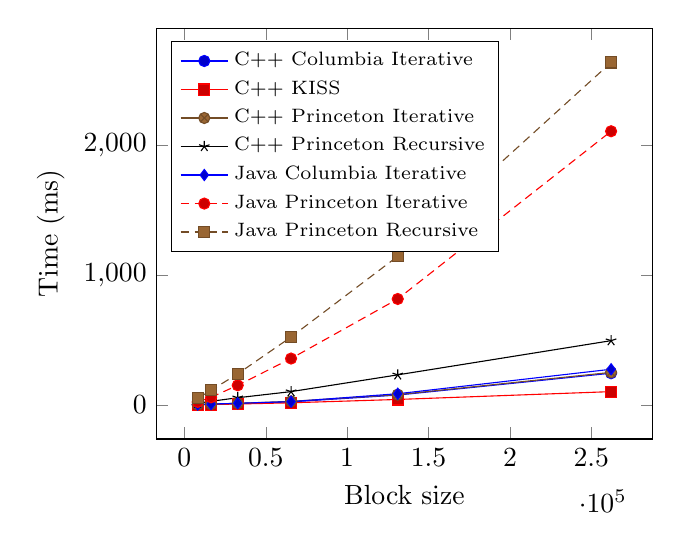
\begin{tikzpicture}
\begin{axis}[xlabel={Block size},ylabel={Time (ms)},width=0.65\linewidth,legend pos=north west,scaled y ticks = false,legend cell align=left,legend style={font=\scriptsize}]
\addplot coordinates {
(8192, 1.9326)
(16384, 4.2789)
(32768, 9.9388)
(65536, 23.1031)
(131072, 75.4942)
(262144, 243.8496)
};
\addplot coordinates {
(8192, 1.2470)
(16384, 2.3713)
(32768, 6.7420)
(65536, 16.0281)
(131072, 41.7620)
(262144, 102.1196)
};
\addplot coordinates {
(8192, 2.5845)
(16384, 5.4518)
(32768, 12.2266)
(65536, 27.2805)
(131072, 78.9501)
(262144, 250.4870)
};
\addplot coordinates {
(8192, 13.2345)
(16384, 27.6080)
(32768, 55.1227)
(65536, 102.1585)
(131072, 231.2663)
(262144, 494.7038)
};
\addplot coordinates {
(8192, 2.8726)
(16384, 6.3214)
(32768, 12.2634)
(65536, 24.9874)
(131072, 85.9483)
(262144, 274.5134)
};
\addplot coordinates {
(8192, 22.9609)
(16384, 58.3825)
(32768, 150.7299)
(65536, 356.9871)
(131072, 815.8607)
(262144, 2108.0771)
};
\addplot coordinates {
(8192, 52.0853)
(16384, 112.3024)
(32768, 239.0777)
(65536, 522.7409)
(131072, 1144.8802)
(262144, 2638.0547)
};
\legend{C++ Columbia Iterative,C++ KISS,C++ Princeton Iterative,C++ Princeton Recursive,Java Columbia Iterative,Java Princeton Iterative,Java Princeton Recursive}
\end{axis}
\end{tikzpicture}

    \caption{Line graph for all algorithms, extra large block sizes}
    \label{fig:all:line:extra}
\end{figure}

